\documentclass[11pt]{article}
\usepackage[margin=0.82in]{geometry}
\usepackage{amsmath,amssymb,booktabs,enumitem,fancyhdr,float,graphicx,microtype,multicol,tabularx,xcolor}
\usepackage[colorlinks=true,urlcolor=blue!50!black,linkcolor=blue!50!black,citecolor=blue!50!black]{hyperref}
\graphicspath{{../../output/tabular/figures/}}
\definecolor{navy}{HTML}{1F4E78}
\definecolor{lightblue}{HTML}{D9EAF7}
\definecolor{lightgray}{HTML}{F2F3F5}
\definecolor{darkgreen}{HTML}{147D64}
\setlength{\parindent}{0pt}
\setlength{\parskip}{5pt}
\setlist[itemize]{itemsep=2pt,topsep=3pt}
\setlist[enumerate]{itemsep=3pt,topsep=3pt}
\pagestyle{fancy}
\setlength{\headheight}{14pt}
\fancyhf{}
\lhead{MATH 550}
\rhead{Modeling Tabular Data}
\cfoot{\thepage}
\newcommand{\E}{\mathbb{E}}
\newcommand{\R}{\mathbb{R}}
\newcommand{\ind}{\mathbb{1}}
\newcommand{\code}[1]{\texttt{#1}}
\newcommand{\aside}[1]{\colorbox{lightblue}{\parbox{0.96\linewidth}{#1}}}
\hypersetup{
  pdftitle={Modeling Tabular Data: Lecture Notes},
  pdfauthor={MATH 550 Capstone Course Development},
  pdfsubject={Transparent logistic regression, tree ensembles, and boosting}
}

\renewcommand{\ind}{\mathbb{I}}

\begin{document}

\begin{center}
{\LARGE\bfseries\color{navy} Modeling Tabular and Structured Data}\\[5pt]
{\Large Logistic regression, regularization, forests, and boosting}\\[8pt]
{\large Detailed lecture notes with scratch-versus-library evidence}\\[10pt]
MATH 550 Mathematical Data Science Capstone
\end{center}

\aside{\textbf{Central lesson.} A high-level estimator is easier to trust after
we can trace its governing objective into primitive code, test the resulting
behavior, and explain any remaining gap. Agreement in ROC AUC verifies ranking;
it does not automatically verify probability calibration, optimization, or
parameter equivalence.}

\tableofcontents
\newpage

\section{Learning objectives and module map}

By the end of the module, students should be able to:

\begin{enumerate}
\item derive binary cross-entropy from a Bernoulli likelihood and implement it
with numerically stable formulas;
\item derive logistic gradients and connect L1/L2 penalties to proximal and
smooth optimization updates;
\item explain and implement CART splitting, bootstrap aggregation, feature
subsampling, and adaptive observation reweighting;
\item interpret gradient boosting as descent in function space and derive the
second-order XGBoost leaf and split equations;
\item explain histogram split search and leaf-wise growth in LightGBM-style
training;
\item conduct a controlled scratch-versus-library comparison on untouched test
data using ranking, threshold, probability, and uncertainty metrics;
\item diagnose discrepancies using mathematical and software mechanisms rather
than declaring one implementation ``wrong'' from a single metric.
\end{enumerate}

The recommended classroom sequence is eight 75-minute meetings. Meetings 1--3
develop logistic regression and regularization; 4--5 develop trees, forests, and
AdaBoost; 6--7 develop first- and second-order boosting; meeting 8 is an evidence
lab using the benchmark outputs. Short code-reading exercises use the modules
listed in Table~\ref{tab:code-map}.

\begin{table}[H]
\centering
\small
\begin{tabularx}{\linewidth}{p{0.25\linewidth}X}
\toprule
File & Teaching responsibility \\
\midrule
\code{models/linear.py} & score, sigmoid, cross-entropy, penalties, accelerated proximal-gradient training, and fitted interfaces \\
\code{models/trees.py} & weighted CART classification, regression trees, and Newton tree nodes \\
\code{models/ensembles.py} & bootstrap/random-feature forests and weighted-stump AdaBoost \\
\code{models/boosting.py} & first-order gradient boosting, exact Newton boosting, and histogram leaf-wise boosting \\
\code{evaluation.py} & binary metrics, probability checks, paired bootstrap, and agreement diagnostics \\
\code{experiments/tabular} & fixed configuration, controlled model pairs, diagnostics, artifact writing, and report generation \\
\bottomrule
\end{tabularx}
\caption{The package is split by mathematical responsibility, not by arbitrary software layers.}
\label{tab:code-map}
\end{table}

\section{The empirical question and public benchmark}

\subsection{Dataset and target}

The classroom benchmark is the Breast Cancer Wisconsin (Diagnostic) dataset
from the UCI Machine Learning Repository \cite{uci-wdbc}. It has 569 rows and 30
continuous features computed from digitized images of a fine needle aspirate of
a breast mass. The features summarize radius, texture, perimeter, area,
smoothness, compactness, concavity, concave points, symmetry, and fractal
dimension. There are no missing values in the bundled copy.

The original labels are malignant and benign. The module explicitly encodes

\[
 y_i = \begin{cases}
 1, & \text{malignant},\\
 0, & \text{benign}.
 \end{cases}
\]

This direction matters: sensitivity is then the fraction of malignant cases
correctly flagged, and the predicted probability is interpreted as the
probability of malignancy. The data are licensed CC BY 4.0 by UCI and loaded
from scikit-learn's local copy, so a benchmark run does not depend on a live
download.

\subsection{A fixed, leakage-resistant protocol}

The experiment uses a class-stratified 80/20 split with random seed 550: 455
training observations and 114 test observations. The split is fixed before
model fitting. Logistic predictors are standardized with means and standard
deviations learned on the training set; tree models use original feature scales.
Any regularization-path comparison uses only a further training/validation split
inside the 455 training rows. The final test set is not a tuning resource.

This design supports a narrow claim: under the documented split and
hyperparameters, does each compact implementation reproduce the relevant
predictive behavior of its production counterpart? It does not establish a
clinical decision rule, population transportability, or superiority among model
families.

\subsection{Why the comparison is paired}

For each family, the scratch and library estimators see the same rows, labels,
preprocessing policy, and nominal hyperparameters. Test AUC differences use
2,000 class-stratified paired-bootstrap samples. A bootstrap replicate samples
positive and negative test indices with replacement, then evaluates both
implementations on exactly the same sampled rows. Pairing removes resampling
variation that would arise if the two models were evaluated on different
replicates.

The pre-declared consistency rule is intentionally practical: a pair is called
performance-consistent when the 95\% paired-bootstrap interval for scratch minus
library AUC contains zero, or the observed absolute AUC gap is no more than 0.02.
This is a teaching tolerance, not a universal equivalence margin.

\section{Evaluation: one metric cannot verify a model}

Let $\hat p_i$ be the predicted probability for class 1 and
$\hat y_i=\ind(\hat p_i\geq 0.5)$.

\subsection{Ranking, thresholds, and probabilities}

\begin{itemize}
\item \textbf{ROC AUC} is the probability that a randomly selected positive
receives a higher score than a randomly selected negative. It is invariant to
strictly increasing transformations of the score.
\item \textbf{Accuracy} is the fraction of correct labels at the chosen
threshold. It can hide class imbalance.
\item \textbf{Sensitivity} is $\mathrm{TP}/(\mathrm{TP}+\mathrm{FN})$ and
\textbf{specificity} is $\mathrm{TN}/(\mathrm{TN}+\mathrm{FP})$.
\item \textbf{Log loss} is
\[
 -\frac1n\sum_{i=1}^n\{y_i\log\hat p_i+(1-y_i)\log(1-\hat p_i)\}.
\]
It strongly penalizes confident mistakes.
\item \textbf{Brier score} is $n^{-1}\sum_i(y_i-\hat p_i)^2$. It evaluates
probability accuracy on a quadratic scale.
\end{itemize}

AUC can agree perfectly while log loss differs: two models can induce the same
ordering but map their margins to different probability ranges. Therefore the
benchmark also reports probability mean absolute error (MAE), probability
correlation, and label agreement between each implementation pair.

\subsection{What a scratch-versus-library gap can mean}

A gap is evidence to investigate, not a verdict. Common mechanisms include:

\begin{itemize}
\item different loss reduction conventions (sum versus mean);
\item a different mapping between $C$ and $\lambda$;
\item penalizing or not penalizing the intercept;
\item different solvers, stopping rules, initialization, or line searches;
\item different random-number streams, tie-breaking, or threshold candidates;
\item optimized terminal-region values in a library boosting implementation;
\item different score-to-probability transformations;
\item production safeguards for missing data, numeric precision, or degenerate
splits that are intentionally absent from a compact teaching implementation.
\end{itemize}

\section{Logistic regression from probability to code}

\subsection{Linear score and sigmoid}

For $x_i\in\R^p$, logistic regression forms the score

\[
 z_i=x_i^\top\beta+b
\]

and applies the sigmoid

\[
 p_i=\sigma(z_i)=\frac{1}{1+e^{-z_i}}.
\]

The log-odds are linear:

\[
 \log\frac{p_i}{1-p_i}=x_i^\top\beta+b.
\]

The decision boundary at probability 0.5 is the hyperplane
$x_i^\top\beta+b=0$. Coefficients describe changes in log-odds for one-unit
feature changes conditional on the other features; they are not automatically
causal effects.

\subsection{Bernoulli likelihood and cross-entropy}

Assume conditionally independent Bernoulli responses:

\[
 p(y_i\mid x_i,\beta,b)=p_i^{y_i}(1-p_i)^{1-y_i}.
\]

The mean negative log-likelihood is

\begin{align*}
\ell(\beta,b)
&=-\frac1n\sum_{i=1}^n\left[y_i\log p_i+(1-y_i)\log(1-p_i)\right]\\
&=\frac1n\sum_{i=1}^n\left[\log(1+e^{z_i})-y_i z_i\right].
\end{align*}

The second form is the one implemented. Computing
\code{logaddexp(0, z)} avoids overflow from explicitly evaluating $e^z$ for a
large positive score. A stable sigmoid uses separate algebra for positive and
negative scores so that $e^{-z}$ or $e^z$ remains bounded.

\subsection{Gradient and curvature}

Because $\partial\ell_i/\partial z_i=p_i-y_i$, the gradient is

\[
 \nabla_\beta\ell=\frac1nX^\top(p-y),
 \qquad
 \frac{\partial\ell}{\partial b}=\frac1n\mathbf{1}^\top(p-y).
\]

Let $\tilde X=[\mathbf{1},X]$ and $w=[b,\beta^\top]^\top$. The Hessian is

\[
 \nabla^2\ell(w)=\frac1n\tilde X^\top W\tilde X,
 \qquad W=\operatorname{diag}\{p_i(1-p_i)\}.
\]

Since $0\le p_i(1-p_i)\le 1/4$, the gradient is Lipschitz with a global bound

\[
 L\le \frac{\lVert\tilde X\rVert_2^2}{4n}.
\]

The scratch optimizer uses $1/L$ as its initial step size. This is slower than a
carefully tuned second-order method but makes the objective-to-update map visible.

\subsection{Reusable estimator interface}

\code{ScratchLogisticRegression} exposes
\code{fit}, \code{decision\_function}, \code{predict\_proba}, and
\code{predict}. It also exposes \code{coef\_}, \code{intercept\_},
\code{loss\_curve\_}, separate data and regularization loss histories,
\code{n\_iter\_}, \code{converged\_}, and the accepted step size. The public
\code{objective\_components} method lets a student verify

\[
 \text{objective}=\text{data loss}+\text{regularization loss}
\]

at the fitted parameters. A finite-difference unit test independently verifies
the analytic gradient.

\section{Regularization and explicit optimization}

\subsection{L2 shrinkage}

The L2 objective is

\[
 F(\beta,b)=\ell(\beta,b)+\frac{\lambda}{2}\lVert\beta\rVert_2^2.
\]

The intercept is not penalized. The gradient contribution is $\lambda\beta$,
and the smooth-gradient update is

\[
 \beta^{(k+1)}=\beta^{(k)}-\eta\left[\frac1nX^\top(p-y)+\lambda\beta^{(k)}\right].
\]

L2 generally shrinks correlated coefficients together. It reduces variance and
prevents coefficients from diverging under complete separation, but it rarely
sets a coefficient exactly to zero.

\subsection{L1 sparsity and the proximal update}

The L1 objective is

\[
 F(\beta,b)=\ell(\beta,b)+\lambda\lVert\beta\rVert_1.
\]

The absolute-value penalty is not differentiable at zero. A proximal-gradient
step first takes a smooth gradient step $u=\beta-\eta\nabla\ell(\beta)$ and then
applies soft thresholding coordinatewise:

\[
 \beta_j^+=\operatorname{sign}(u_j)\max(|u_j|-\eta\lambda,0).
\]

This is not a heuristic zeroing rule. It is the exact proximal operator of the
scaled L1 norm. As $\lambda$ increases, more coordinates cross the threshold and
become exactly zero.

\subsection{Acceleration, restart, and monotone acceptance}

The implementation uses an accelerated proximal-gradient step in the style of
FISTA. Acceleration extrapolates the next search point using the two most recent
accepted iterates. Because extrapolation can overshoot, the implementation
restarts momentum and halves the step until the penalized objective is no larger
than the last accepted value. The recorded objective is therefore monotone up to
floating-point tolerance.

This design serves two teaching goals: students can see a modern first-order
method, and every accepted step remains easy to diagnose. Mature solvers may use
coordinate descent, L-BFGS, trust regions, or screening rules and should be
expected to run faster.

\subsection{Matching scikit-learn's penalty convention}

The scratch objective uses mean loss plus $\lambda\Omega(\beta)$. Scikit-learn's
regularized logistic objective uses a convention equivalent to a summed data
term with inverse strength $C$ for the solvers used here. For $C=1$ and $n$
training observations, the matched scratch value is $\lambda=1/n$. Forgetting
this factor creates a genuine but avoidable parameter gap.

\begin{figure}[H]
\centering
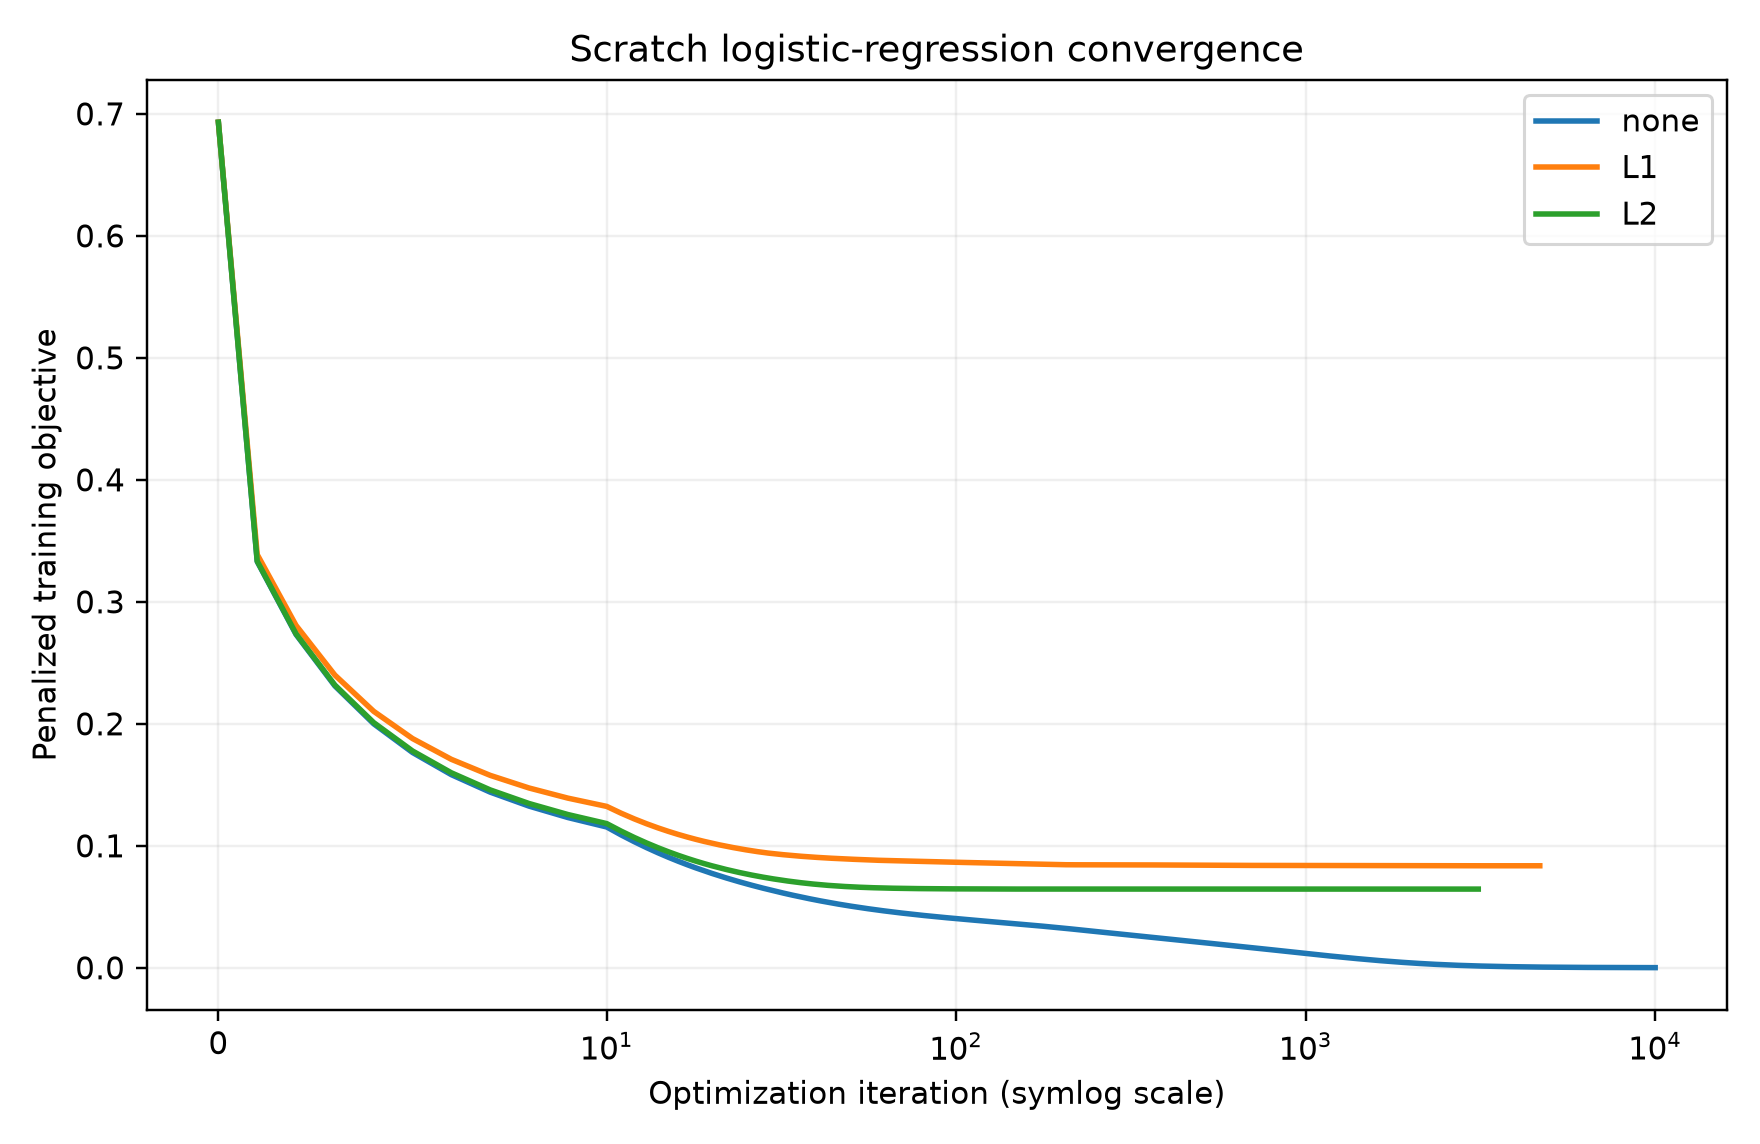
\includegraphics[width=0.79\linewidth]{logistic_optimization.png}
\caption{Accepted penalized-objective paths for the three scratch logistic
models. The plot verifies optimization behavior, not held-out generalization.}
\end{figure}

\begin{figure}[H]
\centering
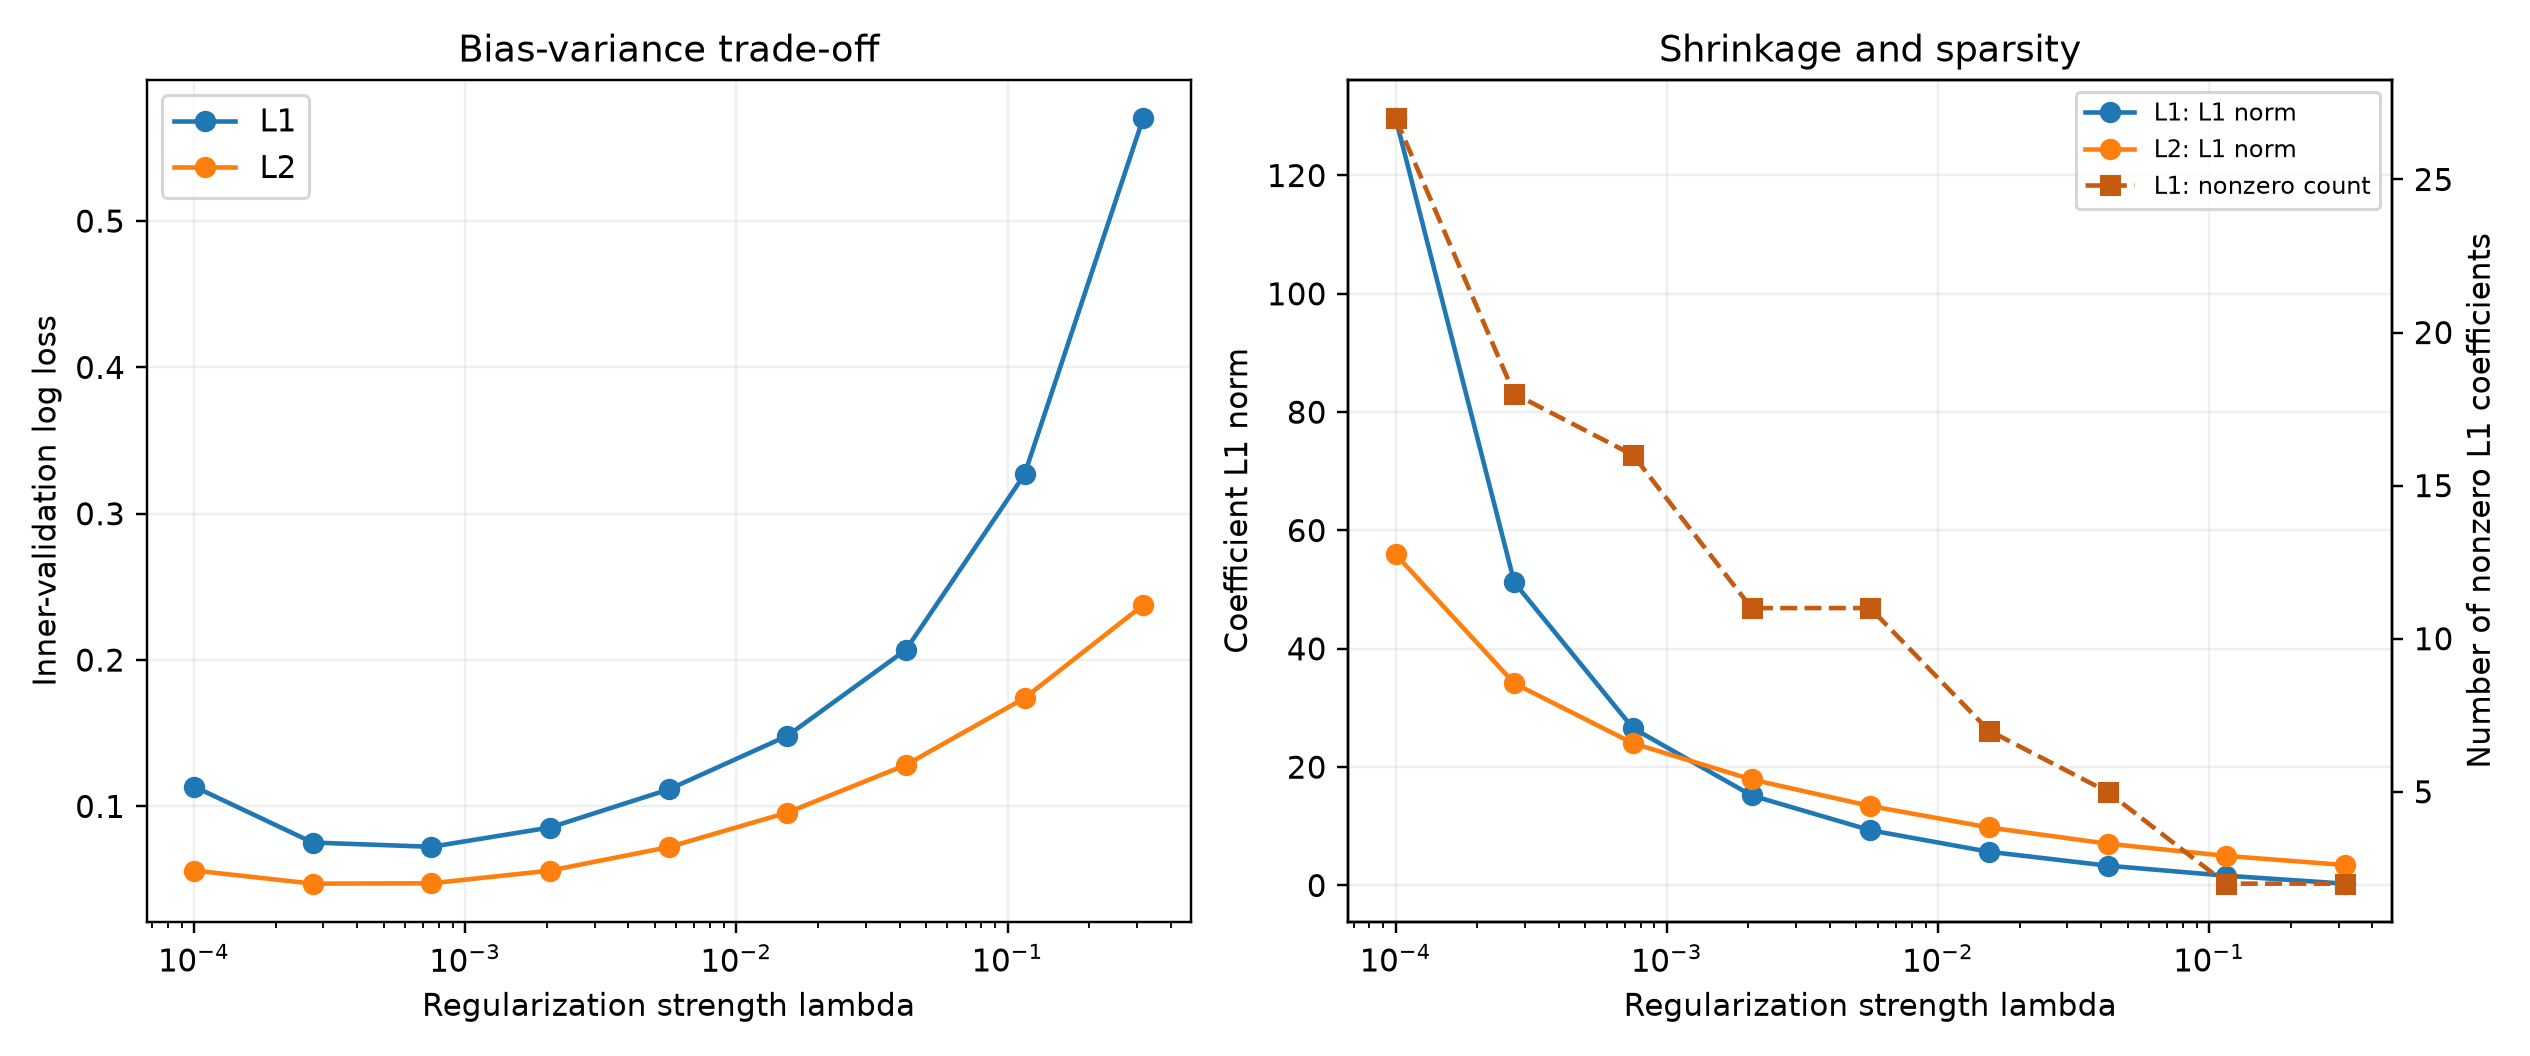
\includegraphics[width=0.96\linewidth]{regularization_effect.png}
\caption{Training-only regularization study. Validation log loss, coefficient
norm, and L1 support answer different questions and are all inspected before the
test set is used.}
\end{figure}

\section{CART: the reusable tree primitive}

\subsection{Weighted Gini splitting}

At a node with nonnegative observation weights $w_i$, define the weighted class
proportion

\[
 \hat\pi_k=\frac{\sum_{i\in\mathcal N}w_i\ind(y_i=k)}
 {\sum_{i\in\mathcal N}w_i}.
\]

Gini impurity is

\[
 I(\mathcal N)=1-\sum_k\hat\pi_k^2.
\]

For split $(j,t)$ with left node $x_{ij}\le t$ and right node $x_{ij}>t$, the
scratch tree minimizes

\[
 Q(j,t)=\frac{W_L}{W}I(\mathcal N_L)+\frac{W_R}{W}I(\mathcal N_R),
\]

subject to leaf-size and depth constraints. Candidate thresholds are midpoints
between sorted distinct observed values. A leaf predicts its weighted positive
fraction, which gives forests an immediate probability interface.

\subsection{Why scaling is unnecessary for an ordinary tree}

A monotone transformation preserves feature order. CART asks which observations
fall to the left or right of a threshold, so multiplying one feature by 1,000
changes the numeric threshold but not the possible partitions. Scaling can still
matter outside the core split rule: numeric precision, downstream distances,
feature engineering, or a mixed pipeline may impose their own requirements.

\subsection{Regression and Newton trees}

First-order gradient boosting reuses a regression tree whose leaf value is the
mean target residual. Second-order boosting uses sums of per-observation
gradients and Hessians. These are separate concise classes because their leaf
objectives are mathematically different, not because an abstract inheritance
hierarchy would look more professional.

\section{Random forests: independent diversity}

A random forest constructs trees independently. For tree $m$:

\begin{enumerate}
\item draw $n$ training rows with replacement;
\item at each node, draw a feature subset, commonly $\sqrt p$ features;
\item fit a CART split using only those candidate features;
\item grow until the depth, leaf-size, or purity rule stops the tree.
\end{enumerate}

The forest probability is the average

\[
 \hat p(x)=\frac1M\sum_{m=1}^M\hat p_m(x).
\]

Bootstrap rows reduce similarity through changed samples; feature subsampling
reduces similarity among strong predictors. Averaging mainly reduces variance.
It does not make each tree unbiased, and feature importance can still be
misleading under correlated predictors.

Matched seeds do not imply identical trees between scratch and scikit-learn.
Libraries consume random numbers in different orders, break ties differently,
and may optimize threshold enumeration. The correct verification target is
controlled predictive behavior and invariants, not byte-for-byte tree identity.

\section{AdaBoost: sequential focus on difficult rows}

AdaBoost is easiest to understand as a \emph{stagewise minimization of
exponential loss}. Represent the labels and each weak classifier by
$\tilde y_i,h_m(x_i)\in\{-1,+1\}$. After $m-1$ rounds, define the ensemble
score

\[
 F_{m-1}(x)=\sum_{k=1}^{m-1}\alpha_k h_k(x).
\]

The predicted class is $\operatorname{sign}(F_{m-1}(x))$, while the magnitude
$|F_{m-1}(x)|$ is a margin measuring confidence on the score scale.

\subsection{Exponential loss and the weighted training sample}

Consider the exponential empirical loss

\[
 \mathcal L(F)=\sum_{i=1}^n \exp\{-\tilde y_i F(x_i)\}.
\]

At round $m$, AdaBoost adds one weak learner with coefficient $\alpha$:

\[
 F_m(x)=F_{m-1}(x)+\alpha h_m(x).
\]

Substituting this stagewise update into the loss gives

\begin{align*}
\mathcal L_m(\alpha)
&=\sum_{i=1}^n
  \exp\{-\tilde y_i[F_{m-1}(x_i)+\alpha h_m(x_i)]\}\\
&=\sum_{i=1}^n
  \underbrace{\exp\{-\tilde y_iF_{m-1}(x_i)\}}_{w_i^{(m)}:\ \text{current difficulty weight}}
  \exp\{-\alpha\tilde y_i h_m(x_i)\}.
\end{align*}

Thus observations with small current margins
$\tilde y_iF_{m-1}(x_i)$ receive relatively large weights. Define the
unnormalized and normalized weights by

\[
 w_i^{(m)}=\exp\{-\tilde y_iF_{m-1}(x_i)\},
 \qquad
 D_i^{(m)}=\frac{w_i^{(m)}}{\sum_{k=1}^n w_k^{(m)}},
 \qquad \sum_i D_i^{(m)}=1.
\]

At the first round, $F_0\equiv0$, so $D_i^{(1)}=1/n$. For a candidate stump
$h_m$, its weighted error is

\[
 \epsilon_m
 =\sum_{i=1}^n D_i^{(m)}\ind\{h_m(x_i)\neq \tilde y_i\}
 =\frac{\sum_i w_i^{(m)}\ind\{h_m(x_i)\neq\tilde y_i\}}
 {\sum_iw_i^{(m)}}.
\]

The weak learner is chosen to make $\epsilon_m$ as small as possible under the
current weights.

\subsection{Deriving the weak-learner coefficient}

For fixed $h_m$, the only remaining scalar decision is $\alpha$. Since
$\tilde y_i h_m(x_i)=+1$ for a correct prediction and $-1$ for a mistake, split
the weighted sum into correct and incorrect observations:

\begin{align*}
\mathcal L_m(\alpha)
&\propto
 \sum_i D_i^{(m)}\exp\{-\alpha\tilde y_i h_m(x_i)\}\\
&=(1-\epsilon_m)e^{-\alpha}+\epsilon_m e^{\alpha}.
\end{align*}

Differentiate with respect to $\alpha$:

\[
 \frac{d\mathcal L_m}{d\alpha}
 =-(1-\epsilon_m)e^{-\alpha}+\epsilon_m e^\alpha.
\]

Setting the derivative to zero gives

\begin{align*}
 \epsilon_m e^{\alpha_m}
 &=(1-\epsilon_m)e^{-\alpha_m},\\
 e^{2\alpha_m}
 &=\frac{1-\epsilon_m}{\epsilon_m},\\
 \alpha_m
 &=\boxed{\frac12\log\frac{1-\epsilon_m}{\epsilon_m}}.
\end{align*}

The second derivative is

\[
 (1-\epsilon_m)e^{-\alpha}+\epsilon_m e^\alpha>0,
\]

so this stationary point is the minimizer. The formula also explains the
behavior directly: if $\epsilon_m<1/2$, then $\alpha_m>0$; if
$\epsilon_m=1/2$, then $\alpha_m=0$ and the learner contributes nothing. A
classifier worse than random can be sign-flipped in the binary setting.

\subsection{Deriving the observation-weight update}

The next-round distribution is obtained from the new exponential-loss factors:

\[
 D_i^{(m+1)}
 =\frac{D_i^{(m)}
 \exp\{-\alpha_m\tilde y_i h_m(x_i)\}}{Z_m},
\]

where $Z_m$ normalizes the weights to sum to one. Hence

\[
 D_i^{(m+1)}\propto
 \begin{cases}
 D_i^{(m)}e^{-\alpha_m}, & h_m(x_i)=\tilde y_i,\\[2mm]
 D_i^{(m)}e^{\alpha_m}, & h_m(x_i)\neq\tilde y_i.
 \end{cases}
\]

Correctly classified observations are downweighted and mistakes are
upweighted. At the minimizing value of $\alpha_m$,

\begin{align*}
 Z_m
 &=(1-\epsilon_m)e^{-\alpha_m}+\epsilon_m e^{\alpha_m}\\
 &=2\sqrt{\epsilon_m(1-\epsilon_m)}.
\end{align*}

Thus $Z_m<1$ whenever the weak learner is better than random. This gives a
compact mathematical explanation for why repeated weak improvements can reduce
the exponential training objective.

The final ensemble score is

\[
 F_M(x)=\sum_{m=1}^M\alpha_m h_m(x),
 \qquad \hat y(x)=\operatorname{sign}(F_M(x)).
\]

There is also a useful population interpretation. If
$\pi(x)=\Pr(\tilde Y=+1\mid X=x)$, then the conditional exponential risk is

\[
 \pi(x)e^{-F(x)}+[1-\pi(x)]e^{F(x)}.
\]

Its minimizer satisfies

\[
 F^*(x)=\frac12\log\frac{\pi(x)}{1-\pi(x)},
 \qquad
 \pi(x)=\sigma\{2F^*(x)\}.
\]

This relation motivates a margin-to-probability transformation, but a finite
AdaBoost fit is not automatically calibrated. Different library conventions
can therefore preserve ranking and labels while producing noticeably different
probabilities.

\section{Gradient boosting: descent in function space}

Gradient boosting replaces AdaBoost's fixed exponential loss with a more
general principle: \emph{take a gradient-descent step in the space of prediction
functions}. Let

\[
 \mathcal R(F)=\frac1n\sum_{i=1}^n \ell\bigl(y_i,F(x_i)\bigr)
\]

be the empirical risk for a differentiable loss $\ell$. At iteration $m$, the
current function is $F_{m-1}$.

\subsection{From ordinary gradient descent to a functional gradient}

For an ordinary parameter vector $\theta$, gradient descent uses
$\theta\leftarrow\theta-\eta\nabla_\theta\mathcal R$. Here the trainable object
is a function. At the observed inputs, the analogous negative-gradient values
are

\[
 r_{im}
 =-\left.
 \frac{\partial\ell(y_i,F)}{\partial F}
 \right|_{F=F_{m-1}(x_i)},
 \qquad i=1,\ldots,n.
\]

These $r_{im}$ are called \emph{pseudo-residuals}: they are residual-like
quantities defined by the loss gradient, not necessarily by $y_i-F(x_i)$.
Because the next step is restricted to a class of shallow regression trees
$\mathcal H$, gradient boosting approximates this negative-gradient vector by
solving

\[
 f_m\approx
 \arg\min_{f\in\mathcal H}
 \sum_{i=1}^n\{r_{im}-f(x_i)\}^2.
\]

The update is then

\[
 \boxed{F_m(x)=F_{m-1}(x)+\eta f_m(x)},
\]

where $0<\eta\le 1$ is the learning rate. The tree is therefore a structured
approximation to the steepest-descent direction.

\subsection{Binary cross-entropy pseudo-residuals}

For binary classification with $y_i\in\{0,1\}$, use the score-scale logistic
loss

\[
 \ell(y_i,F_i)=\log(1+e^{F_i})-y_iF_i,
 \qquad p_i=\sigma(F_i).
\]

Differentiate step by step:

\begin{align*}
 \frac{\partial\ell_i}{\partial F_i}
 &=\frac{e^{F_i}}{1+e^{F_i}}-y_i\\
 &=\sigma(F_i)-y_i\\
 &=p_i-y_i.
\end{align*}

Hence the negative gradient is

\[
 \boxed{r_{im}=y_i-p_i},
 \qquad p_i=\sigma\{F_{m-1}(x_i)\}.
\]

An observation with $y_i=1$ but a small predicted probability has a large
positive pseudo-residual, so the next tree tries to increase its score. An
observation with $y_i=0$ but a large predicted probability has a large negative
pseudo-residual, so the next tree tries to decrease its score.

\subsection{Deriving the initial constant score}

Before fitting any tree, choose the best constant score

\[
 F_0(x)\equiv c^*
 =\arg\min_c\sum_{i=1}^n
 \left[\log(1+e^c)-y_ic\right].
\]

Let $\bar y=n^{-1}\sum_i y_i$. Differentiating gives

\begin{align*}
 0
 &=\sum_{i=1}^n\{\sigma(c^*)-y_i\}\\
 &=n\{\sigma(c^*)-\bar y\}.
\end{align*}

Therefore $\sigma(c^*)=\bar y$, and

\[
 \boxed{F_0=\log\frac{\bar y}{1-\bar y}}.
\]

Thus boosting starts from the training-set log-odds and lets subsequent trees
model deviations from that constant baseline.

\subsection{Why a regression-tree leaf stores a mean pseudo-residual}

Suppose the fitted tree partitions the input space into terminal regions
$R_{1m},\ldots,R_{J_m m}$. If a leaf $R_{jm}$ stores a constant $c_{jm}$ and the
tree is fitted by least squares to the pseudo-residuals, then

\[
 c_{jm}
 =\arg\min_c\sum_{i:x_i\in R_{jm}}(r_{im}-c)^2.
\]

Differentiate:

\[
 -2\sum_{i:x_i\in R_{jm}}(r_{im}-c)=0,
\]

so

\[
 \boxed{c_{jm}
 =\frac{1}{|R_{jm}|}\sum_{i:x_i\in R_{jm}}r_{im}}.
\]

This is the leaf rule used by the compact first-order implementation: each leaf
stores the mean pseudo-residual, and

\[
 f_m(x)=\sum_{j=1}^{J_m}c_{jm}\ind\{x\in R_{jm}\}.
\]

\subsection{Optional terminal-region optimization and the bridge to Newton boosting}

After a tree structure has been chosen, a more aggressive implementation can
optimize a separate score increment $\gamma_{jm}$ inside each leaf:

\[
 \gamma_{jm}
 =\arg\min_\gamma
 \sum_{i:x_i\in R_{jm}}
 \ell\bigl(y_i,F_{m-1}(x_i)+\gamma\bigr).
\]

For logistic loss this one-dimensional problem does not simplify to the mean
pseudo-residual. A second-order approximation around $\gamma=0$ gives

\[
 \ell_i(F_i+\gamma)
 \approx \ell_i(F_i)+g_i\gamma+\frac12h_i\gamma^2,
\]

with

\[
 g_i=p_i-y_i,
 \qquad
 h_i=p_i(1-p_i).
\]

Within one leaf, differentiating the quadratic approximation yields

\begin{align*}
 0
 &\approx\sum_{i\in R_{jm}}(g_i+h_i\gamma_{jm}),\\
 \gamma_{jm}
 &\approx-\frac{\sum_{i\in R_{jm}}g_i}
 {\sum_{i\in R_{jm}}h_i}\\
 &=\frac{\sum_{i\in R_{jm}}(y_i-p_i)}
 {\sum_{i\in R_{jm}}p_i(1-p_i)}.
\end{align*}

This calculation is the direct bridge from first-order gradient boosting to the
second-order, Newton-style leaf values used by XGBoost-style methods. It also
explains why two implementations can fit very similar rankings while producing
different probability scales: mean pseudo-residual leaves and optimized
terminal values are different numerical updates.

\section{XGBoost-style second-order trees}

XGBoost-style boosting keeps the additive-tree structure of gradient boosting
but uses a second-order approximation to the loss and an explicit tree
regularizer. Let the current score be $F_{m-1}(x)$ and add a new tree $f_m$:

\[
 F_m(x)=F_{m-1}(x)+\eta f_m(x).
\]

For deriving the tree itself, temporarily set aside the learning-rate factor
$\eta$ and optimize the unshrunk increment $f=f_m$.

\subsection{Step 1: write the regularized stagewise objective}

At iteration $m$, the part of the training objective involving the new tree is

\[
 \mathcal J^{(m)}
 =\sum_{i=1}^n
 \ell\bigl(y_i,F_{m-1}(x_i)+f(x_i)\bigr)+\Omega(f),
\]

with tree regularization

\[
 \Omega(f)=\gamma T+\frac\lambda2\sum_{j=1}^T w_j^2.
\]

Here $T$ is the number of terminal leaves, $w_j$ is the score stored in leaf
$j$, $\gamma\ge0$ penalizes adding leaves, and $\lambda\ge0$ applies L2
shrinkage to leaf scores.

\subsection{Step 2: take a second-order Taylor expansion}

Write $F_i=F_{m-1}(x_i)$ and $f_i=f(x_i)$. Around the current score $F_i$,

\[
 \ell(y_i,F_i+f_i)
 \approx
 \ell(y_i,F_i)+g_i f_i+\frac12 h_i f_i^2,
\]

where

\[
 g_i=\left.\frac{\partial\ell(y_i,F)}{\partial F}\right|_{F=F_i},
 \qquad
 h_i=\left.\frac{\partial^2\ell(y_i,F)}{\partial F^2}\right|_{F=F_i}.
\]

For logistic loss,

\begin{align*}
 \ell(y_i,F_i)
 &=\log(1+e^{F_i})-y_iF_i,\\
 g_i
 &=\frac{e^{F_i}}{1+e^{F_i}}-y_i
 =p_i-y_i,\\
 h_i
 &=\frac{d}{dF_i}\sigma(F_i)
 =p_i(1-p_i).
\end{align*}

The terms $\ell(y_i,F_i)$ do not depend on the new tree, so they can be dropped
when comparing candidate trees. The approximate objective becomes

\[
 \widetilde{\mathcal J}^{(m)}(f)
 =\sum_{i=1}^n
 \left[g_i f(x_i)+\frac12h_i f(x_i)^2\right]
 +\gamma T+\frac\lambda2\sum_{j=1}^T w_j^2.
\]

\subsection{Step 3: group observations by tree leaf}

Let $q(x)\in\{1,\ldots,T\}$ map an observation to its leaf and write

\[
 f(x)=w_{q(x)}.
\]

For leaf $j$, define its index set and accumulated first- and second-order
statistics

\[
 I_j=\{i:q(x_i)=j\},
 \qquad
 G_j=\sum_{i\in I_j}g_i,
 \qquad
 H_j=\sum_{i\in I_j}h_i.
\]

Then

\begin{align*}
\widetilde{\mathcal J}^{(m)}
&=\sum_{j=1}^T
 \left[
 \sum_{i\in I_j}g_i w_j
 +\frac12\sum_{i\in I_j}h_i w_j^2
 +\frac\lambda2w_j^2
 \right]+\gamma T\\
&=\sum_{j=1}^T
 \left[G_jw_j+\frac12(H_j+\lambda)w_j^2\right]
 +\gamma T.
\end{align*}

Once the tree structure is fixed, the leaf weights separate: each $w_j$ can be
optimized independently.

\subsection{Step 4: derive the optimal leaf value}

For one leaf, minimize

\[
 \phi_j(w)=G_jw+\frac12(H_j+\lambda)w^2.
\]

Differentiate and set to zero:

\begin{align*}
 \phi_j'(w)
 &=G_j+(H_j+\lambda)w=0,\\
 w_j^*
 &=\boxed{-\frac{G_j}{H_j+\lambda}}.
\end{align*}

The same result can be seen by completing the square:

\[
 \phi_j(w)
 =\frac12(H_j+\lambda)
 \left(w+\frac{G_j}{H_j+\lambda}\right)^2
 -\frac12\frac{G_j^2}{H_j+\lambda}.
\]

Therefore the optimized contribution of leaf $j$ is

\[
 \phi_j(w_j^*)=-\frac12\frac{G_j^2}{H_j+\lambda}.
\]

For a fixed tree structure $q$, the optimized approximate objective is thus

\[
 \boxed{
 \widetilde{\mathcal J}^{(m)}(q)
 =-\frac12\sum_{j=1}^T\frac{G_j^2}{H_j+\lambda}
 +\gamma T
 }
\]

up to the dropped constant from the previous ensemble.

\subsection{Step 5: derive the split-gain formula}

Suppose a parent leaf with statistics $(G_P,H_P)$ is split into left and right
children. Since the children partition the parent,

\[
 G_P=G_L+G_R,
 \qquad
 H_P=H_L+H_R.
\]

Before the split, the optimized parent contribution is

\[
 -\frac12\frac{G_P^2}{H_P+\lambda}+\gamma.
\]

After the split, the two optimized child contributions are

\[
 -\frac12\frac{G_L^2}{H_L+\lambda}
 -\frac12\frac{G_R^2}{H_R+\lambda}
 +2\gamma.
\]

Define gain as ``objective before minus objective after.'' Then

\begin{align*}
\mathrm{Gain}
&=\frac12\left[
 \frac{G_L^2}{H_L+\lambda}
 +\frac{G_R^2}{H_R+\lambda}
 -\frac{G_P^2}{H_P+\lambda}
 \right]-\gamma\\
&=\boxed{
 \frac12\left[
 \frac{G_L^2}{H_L+\lambda}
 +\frac{G_R^2}{H_R+\lambda}
 -\frac{(G_L+G_R)^2}{H_L+H_R+\lambda}
 \right]-\gamma}.
\end{align*}

A split is useful only when the reduction in the quadratic loss approximation
is large enough to pay the extra leaf penalty $\gamma$.

\subsection{Interpretation and relation to Newton's method}

The gradient sum $G_j$ determines the direction in which a leaf score should
move. The Hessian sum $H_j$ measures local curvature: when curvature is large,
a given gradient produces a smaller Newton step. The regularizer $\lambda$
further shrinks the leaf value and prevents unstable updates when $H_j$ is
small.

If $\lambda=0$, then

\[
 w_j^*=-\frac{G_j}{H_j}
\]

is exactly the Newton step for a constant score increment within that leaf.
XGBoost-style training can therefore be viewed as repeatedly constructing a
tree-structured approximation to a Newton step, followed by shrinkage through
the learning rate $\eta$. Minimum child weight, row subsampling, and column
subsampling provide additional regularization.

The scratch version enumerates exact observed thresholds. Production XGBoost
uses a histogram engine in the matched reference configuration and adds missing
value logic, parallelism, memory optimizations, and numerical safeguards
\cite{xgboost}.

\section{LightGBM-style histograms and leaf-wise growth}

Exact split search repeatedly considers many observed feature values. Histogram
training first maps continuous values into a fixed number of ordered bins. It
then accumulates gradient and Hessian sums per bin and evaluates only bin
boundaries. With $B\ll n$ bins, split search can be much cheaper and cache
friendlier, at the price of quantizing thresholds.

Depth-wise growth expands nodes level by level. Leaf-wise growth maintains all
current leaves, evaluates their best available splits, and expands the globally
highest-gain leaf. This can reduce training loss quickly for a fixed number of
leaves, but on a small dataset it can create an uneven, highly specialized
branch. The scratch class therefore exposes both \code{num\_leaves} and
\code{max\_depth}.

The classroom implementation captures quantile bins, gradient/Hessian
histograms, and best-leaf-first growth. It does not reproduce distributed
training, exclusive feature bundling, gradient-based one-side sampling,
categorical-feature algorithms, or every production missing-value behavior
described by Ke et al. \cite{lightgbm}.

\section{Measured scratch-versus-library results}

\subsection{Held-out ranking consistency}

All eight pre-declared pairs meet the AUC consistency rule. Table~\ref{tab:auc}
reports the untouched 114-row test set. The largest observed absolute gap is
0.006 for unregularized logistic regression; its interval includes zero.

\begin{table}[H]
\centering
\small
\begin{tabular}{lrrrr}
\toprule
Family & Scratch AUC & Library AUC & Gap & 95\% paired interval \\
\midrule
Logistic none & 0.984 & 0.977 & +0.006 & $[-0.002,\ 0.024]$ \\
Logistic L1 & 0.990 & 0.991 & -0.001 & $[-0.004,\ 0.000]$ \\
Logistic L2 & 0.989 & 0.989 & 0.000 & $[0.000,\ 0.000]$ \\
Random forest & 0.991 & 0.992 & -0.001 & $[-0.006,\ 0.002]$ \\
AdaBoost & 0.993 & 0.993 & 0.000 & $[0.000,\ 0.000]$ \\
Gradient boosting & 0.992 & 0.994 & -0.002 & $[-0.009,\ 0.005]$ \\
XGBoost style & 0.993 & 0.991 & +0.002 & $[-0.000,\ 0.007]$ \\
LightGBM style & 0.993 & 0.994 & -0.002 & $[-0.006,\ 0.001]$ \\
\bottomrule
\end{tabular}
\caption{Scratch minus library ROC AUC under the fixed paired protocol.}
\label{tab:auc}
\end{table}

\begin{figure}[H]
\centering
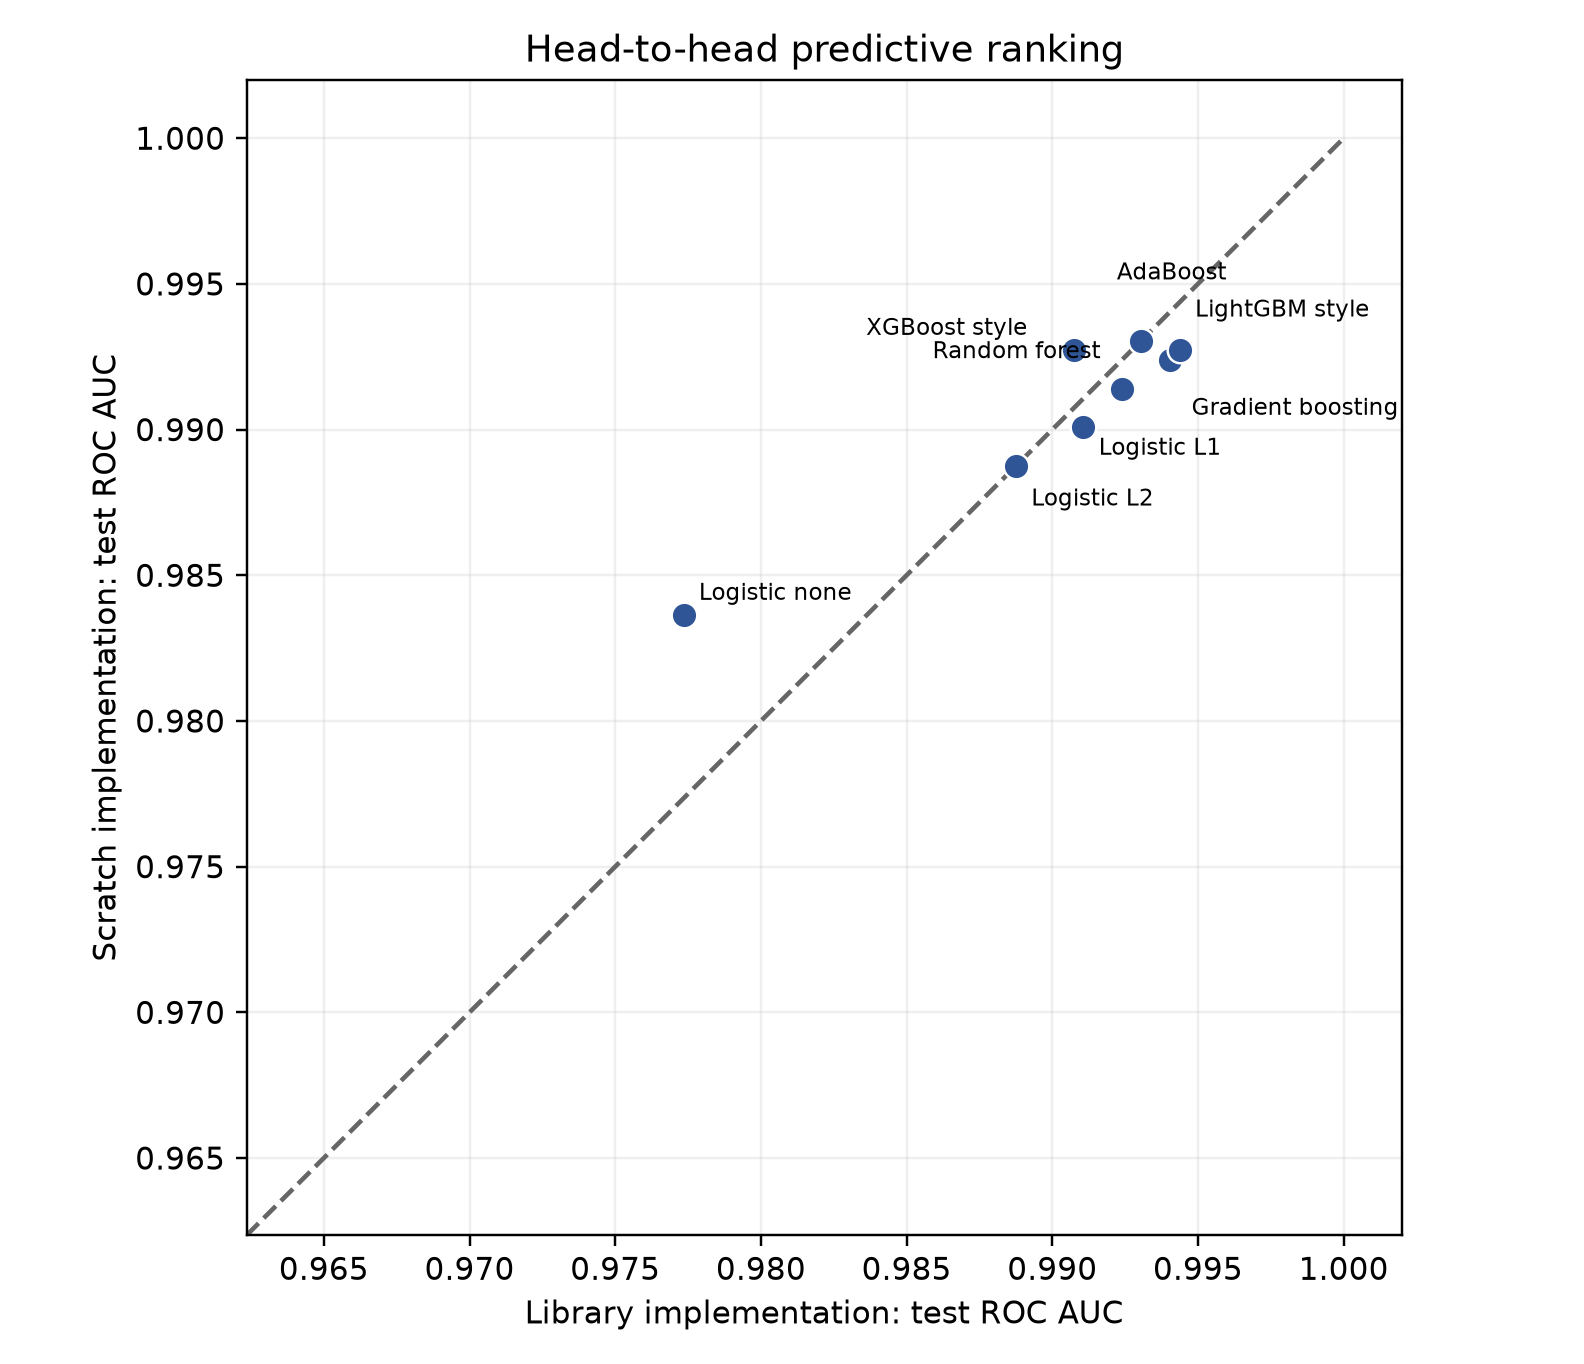
\includegraphics[width=0.73\linewidth]{head_to_head_auc.png}
\caption{Points near the diagonal show held-out ranking consistency. The plot
does not establish calibration equivalence.}
\end{figure}

\begin{figure}[H]
\centering
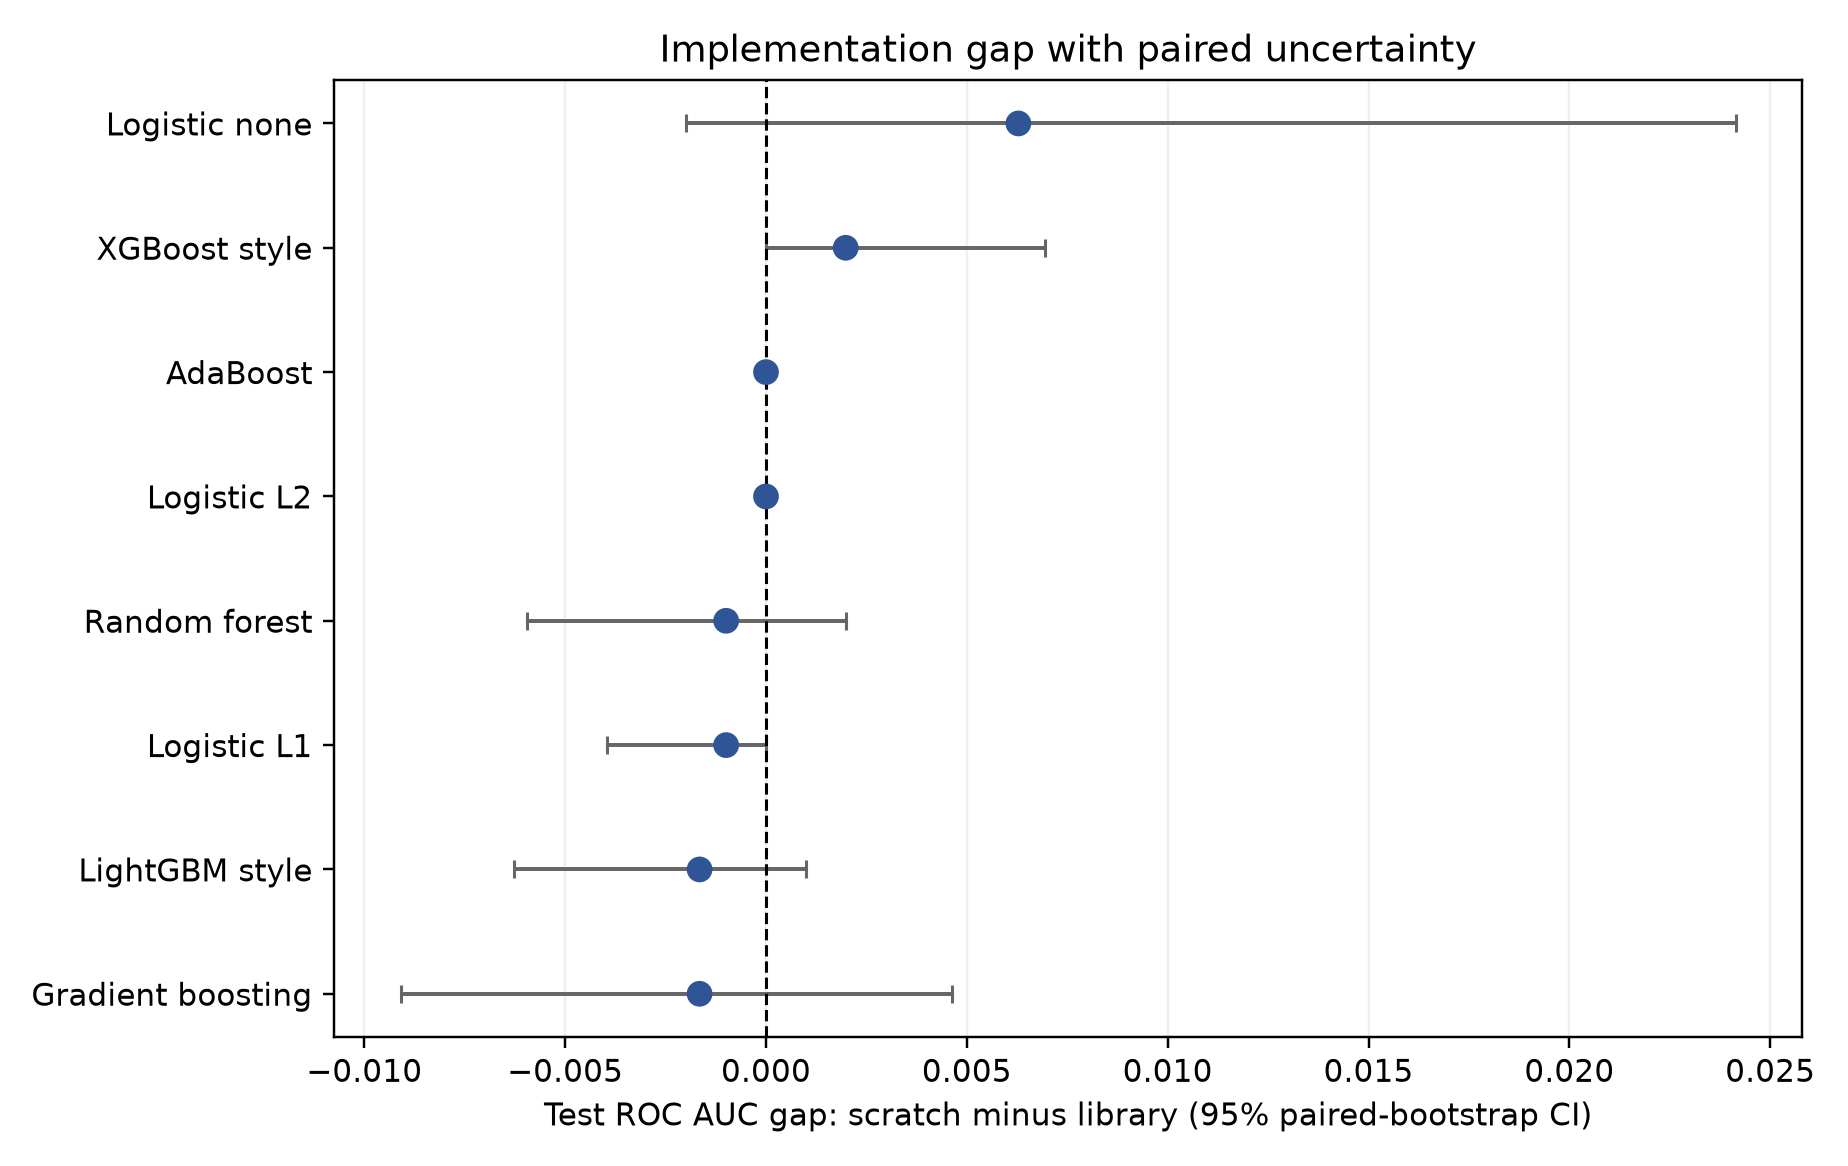
\includegraphics[width=0.88\linewidth]{paired_auc_gaps.png}
\caption{Class-stratified paired-bootstrap intervals quantify uncertainty in
each scratch-minus-library AUC gap.}
\end{figure}

\subsection{Probability discrepancies are the main teaching result}

\begin{table}[H]
\centering
\small
\begin{tabular}{lrrrr}
\toprule
Family & Label agreement & Probability MAE & Scratch log loss & Library log loss \\
\midrule
Logistic none & 0.982 & 0.014 & 0.725 & 0.634 \\
Logistic L1 & 1.000 & 0.005 & 0.095 & 0.088 \\
Logistic L2 & 1.000 & $<10^{-6}$ & 0.099 & 0.099 \\
Random forest & 0.991 & 0.015 & 0.107 & 0.101 \\
AdaBoost & 1.000 & 0.293 & 0.118 & 0.375 \\
Gradient boosting & 0.956 & 0.138 & 0.217 & 0.082 \\
XGBoost style & 0.991 & 0.006 & 0.087 & 0.094 \\
LightGBM style & 0.982 & 0.012 & 0.090 & 0.095 \\
\bottomrule
\end{tabular}
\caption{Agreement in ranking or labels need not imply agreement in probability scale.}
\end{table}

AdaBoost is the cleanest example: AUC and thresholded labels agree exactly, yet
probability MAE is 0.293. The versions use different margin-to-probability
conventions. This supports ranking consistency and label consistency under the
chosen threshold, but not probability equivalence.

Gradient boosting has a smaller AUC gap but a probability MAE of 0.138. Its
mechanism is different: the scratch version stores raw pseudo-residual means,
whereas the library optimizes terminal-region values. Here the data support
similar ranking but materially different confidence.

\begin{figure}[H]
\centering
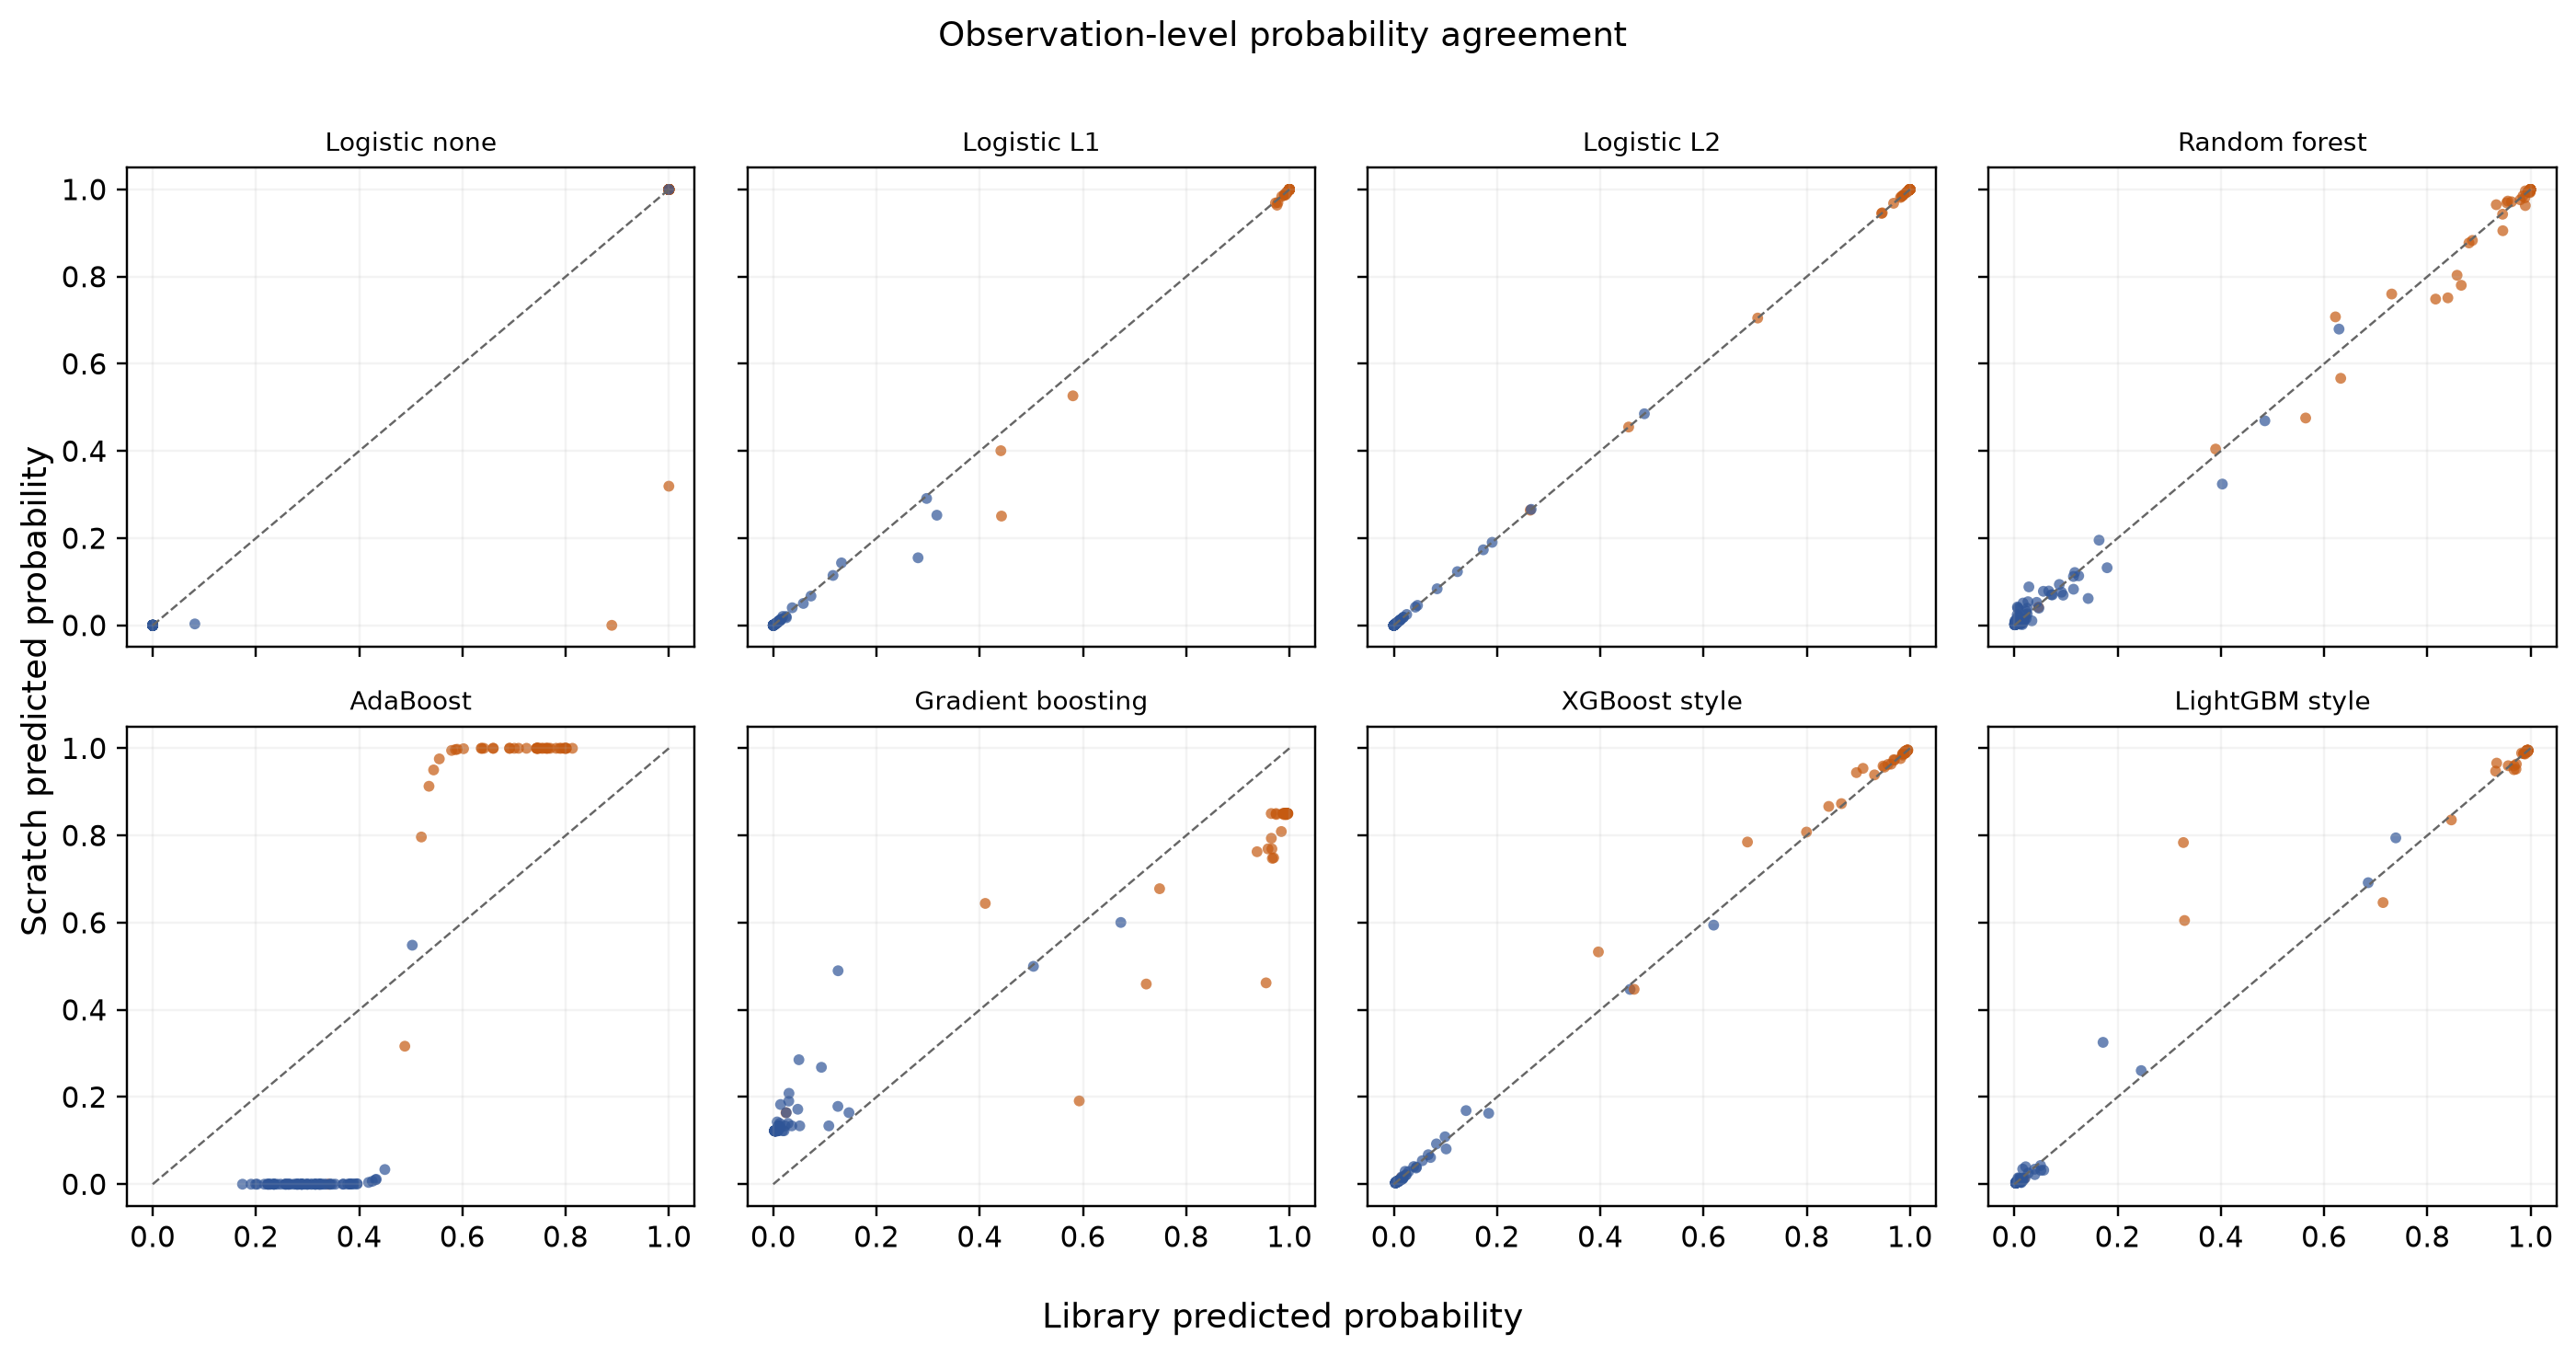
\includegraphics[width=0.98\linewidth]{probability_agreement.png}
\caption{Observation-level probability comparisons reveal transformation and
terminal-value differences that AUC hides.}
\end{figure}

\subsection{The unregularized separation warning}

The 455-row standardized training sample is separable. Unregularized logistic
cross-entropy therefore has an infimum of zero but no finite coefficient
minimizer: scaling a separating direction makes the training loss progressively
smaller. The scratch method reaches its iteration budget rather than satisfying
a finite-parameter convergence rule. The library also produces very large
scores under its solver rules.

Ranking remains strong, but a few confident test mistakes yield log losses of
0.725 and 0.634. L1 and L2 fits have test log losses below 0.10. The lesson is
not that logistic regression failed; it is that unpenalized maximum likelihood
is ill-posed under separation and ranking can conceal extreme probabilities.

\subsection{Parameter verification}

The matched L2 objectives agree to displayed numerical precision, test
probabilities differ by less than $10^{-6}$ on average, and coefficient
correlation exceeds 0.98 in the unit test. L1 is more solver-sensitive near the
selection boundary: standardized coefficient correlation is 0.835, mean
absolute coefficient difference is 0.178, and support Jaccard similarity is
0.938. These results are consistent with matching the same nonsmooth objective
up to solver tolerance while some near-zero coefficients remain unstable.

\section{How to interpret model choice responsibly}

The fixed results do not justify selecting the row with the highest AUC. The
test set has only 42 positive and 72 negative observations, so apparent
differences of a few thousandths are not stable evidence of broad superiority.
The following questions are more useful:

\begin{enumerate}
\item Is the target scientifically and operationally meaningful?
\item Which errors matter, and does threshold 0.5 reflect those costs?
\item Are calibrated probabilities needed, or is ranking enough?
\item Does the new population match the training population and measurement
process?
\item Is a compact linear model adequate, or do nonlinear interactions have a
credible role?
\item Can the pipeline be reproduced, monitored, and independently validated?
\end{enumerate}

For this benchmark, regularized logistic regression is a strong default: it is
compact, stable, and almost indistinguishable from the library reference. Tree
ensembles provide a useful nonlinear comparison. Any deployment would still
need calibration assessment, threshold selection under explicit costs, external
validation, drift monitoring, and human review. The dataset is a classroom
benchmark, not a clinical validation study.

\section{Common failure modes and diagnostic questions}

\begin{tabularx}{\linewidth}{p{0.25\linewidth}X}
\toprule
Symptom & Questions to ask \\
\midrule
Loss becomes NaN & Was sigmoid or cross-entropy implemented stably? Are inputs finite? Is the step too large? \\
Scratch L2 differs strongly & Are features standardized identically? Is $\lambda=1/(nC)$ under the chosen conventions? Is the intercept excluded? \\
L1 support differs & Are near-zero tolerances comparable? Did both solvers converge? Is the objective scaled identically? \\
Forest trees differ & Are predictive metrics and invariants stable despite different random streams and tie-breaking? \\
AUC agrees, log loss differs & Is the margin-to-probability mapping different? Are terminal leaf values optimized differently? \\
Training metric is perfect & Was the test set untouched? Is the model separated or overfit? What do probability metrics show? \\
Fast library, slow scratch & Which production optimizations are absent, and does runtime affect the mathematical verification claim? \\
\bottomrule
\end{tabularx}

\section{Extensions}

Natural extensions include multinomial logistic regression, class/sample
weights, missing-data policies, native categorical splits, monotonic
constraints, calibration curves, threshold selection, partial dependence,
permutation importance, SHAP-style explanations, nested cross-validation, and
external validation. These should be introduced as new lessons with explicit
assumptions rather than quietly folded into the core classes.

For a structured-data sequel, students can compare one-hot encoded linear
models with native categorical boosting, or study grouped and temporal splits
where row-wise random splitting would leak information. The same verification
principle applies: expose the governing mechanism, control the comparison, and
diagnose the dimensions of agreement separately.

\appendix
\section{Pseudocode}

\subsection{Accelerated proximal logistic training}

\begin{enumerate}
\item Form $\tilde X=[\mathbf{1},X]$ and initialize $w=0$, extrapolated point
$v=w$, and momentum $t=1$.
\item Compute the smooth gradient at $v$.
\item Take $u=v-\eta\nabla\ell(v)$, including the L2 gradient when relevant.
\item For L1, soft-threshold coefficient coordinates of $u$; never threshold
the intercept.
\item If the objective increased, restart at $w$ and backtrack $\eta$.
\item Record data loss, penalty, and total objective.
\item Stop when $\lVert u-w\rVert\le\text{tol}(1+\lVert w\rVert)$; otherwise
form the accelerated extrapolation and continue.
\end{enumerate}

\subsection{Random forest}

\begin{enumerate}
\item For $m=1,\ldots,M$, sample training row indices with replacement.
\item Grow a weighted CART tree; at every node sample a feature subset.
\item Store the weighted positive proportion in each leaf.
\item Average the $M$ positive-class probabilities at prediction time.
\end{enumerate}

\subsection{Newton boosting}

\begin{enumerate}
\item Initialize the score with the training log-odds.
\item At round $m$, compute $p=\sigma(F)$, $g=p-y$, and $h=p(1-p)$.
\item Optionally subsample rows and columns.
\item Grow a tree using regularized second-order split gain.
\item Store $-G/(H+\lambda)$ in each leaf.
\item Update $F\leftarrow F+\eta f_m$.
\end{enumerate}

\section{Reproducibility commands}

\begin{verbatim}
uv sync --locked --extra tabular
DYLD_LIBRARY_PATH=.local/libomp/18.1.5/lib make benchmark-tabular
DYLD_LIBRARY_PATH=.local/libomp/18.1.5/lib make validate-homework-tabular
make notes-tabular
make homework-tabular
make verify-slides-tabular
make test
\end{verbatim}

The explicit OpenMP path is needed only on a compatible Apple Silicon setup
where XGBoost/LightGBM cannot find the runtime automatically. A normal system
installation can use its own documented path.

\begin{thebibliography}{9}
\bibitem{uci-wdbc}
W. Wolberg, O. Mangasarian, N. Street, and W. Street.
\emph{Breast Cancer Wisconsin (Diagnostic)}. UCI Machine Learning Repository,
DOI: \href{https://doi.org/10.24432/C5DW2B}{10.24432/C5DW2B}.

\bibitem{breiman}
L. Breiman. Random Forests. \emph{Machine Learning}, 45:5--32, 2001.
DOI: \href{https://doi.org/10.1023/A:1010933404324}{10.1023/A:1010933404324}.

\bibitem{adaboost}
Y. Freund and R. Schapire. A Decision-Theoretic Generalization of On-Line
Learning and an Application to Boosting. \emph{Journal of Computer and System
Sciences}, 55(1):119--139, 1997.

\bibitem{friedman}
J. Friedman. Greedy Function Approximation: A Gradient Boosting Machine.
\emph{Annals of Statistics}, 29(5):1189--1232, 2001.

\bibitem{xgboost}
T. Chen and C. Guestrin. XGBoost: A Scalable Tree Boosting System.
\emph{Proceedings of KDD}, 2016. DOI:
\href{https://doi.org/10.1145/2939672.2939785}{10.1145/2939672.2939785}.

\bibitem{lightgbm}
G. Ke et al. LightGBM: A Highly Efficient Gradient Boosting Decision Tree.
\emph{Advances in Neural Information Processing Systems}, 2017.
\end{thebibliography}

\end{document}
